% !TEX encoding = UTF-8 Unicode
% !TEX root = rapport.tex

\part{Initiatives et solutions}\label{initiatives_actuelles}

\chapter{Initiatives des pouvoirs publics}
\label{sec:initialivespublic}

\section{Mesures des pouvoirs publics français}

\subsection{Le C2i}
Mis en place à partir de la rentrée universitaire 2003 \cite{circulaire_c2i}, le certificat informatique et internet (C2i) vise à encadrer la formation des étudiants aux technologies informatisées et à internet par l'établissement d'un socle commun.

\begin{figure}[H]
  \centering
  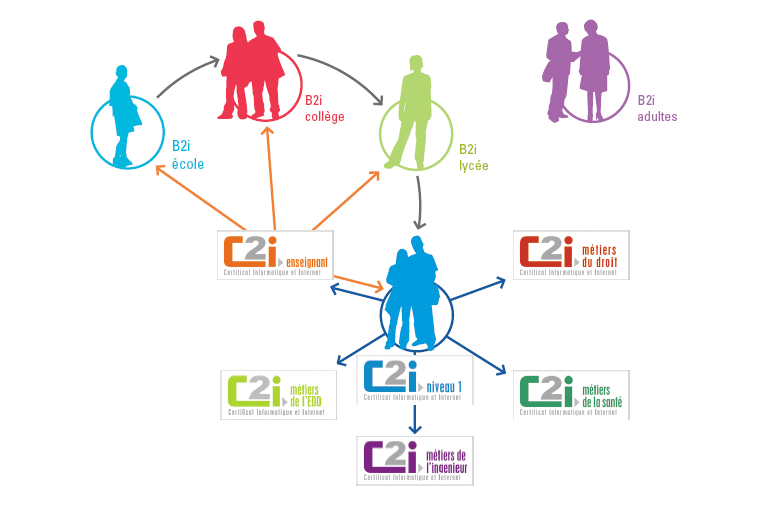
\includegraphics[width=\textwidth]{../resources/illustrations/c2i}
  \caption{Différents niveaux et spécialités du C2i}
\end{figure}

\cite{b2i_c2i}
\cite{b2i}
\cite{isn}

\subsection{Les opérations "ordinateurs portables"}

Les opérations \og{}ordinateurs portables\fg{} sont à la mode au lycée. OrdiLib' en Midi-Pyrénées, Ordipass en Pays de la Loire, LoRdi en Languedoc-Roussilon, ces initiatives des régions visent à fournir à chaque lycéen l'accès à un ordinateur portable personnel.

\cite{portables35}
\cite{portables60}
\cite{portables40}


\subsection{Le rapport \og{}Refondons l'école de la république\fg{}}

Nous avons vu différentes actions mené par le gouvernement ou les régions afin d'une part de former les étudiants au NTIC et d'autres part de favoriser l'utilisation des NTIC dans le système éducatif. Nous allons maintenant nous intéresser aux propositions pour l'avenir de l'éducation à travers la concertation \og{}Refondons l'école de la république\fg{} confié par le gouvernement Ayrault à Nathalie Mons, Christian Forestier, François Bonneau et Marie-Françoise Colombani. Il ressort à travers se rapport plusieurs thèmes tels que \og{}apprendre à apprendre\fg{}, \og{}une appropriation active des langues\fg{}, \og{}usages pédagogiques du numérique en primaire\fg{}, \og{}une évaluation positive, plutôt qu'une note sanction\fg{}… Ces différents thèmes sont des points d'interrogation cruciaux pour l'école de demain, nous regretterons cependant un manque de mesures concrètes. Nous pouvons tout de même relevé la volonté d'inscrire dans la loi \og l'éducation au médias et à l'information\fg{}, de mettre en place un plan pour l'éducation numérique au primaire, de former les enseignants aux usages pédagogiques du numérique, de mettre en place une politique publique de recherche dans le cadre des applications pédagogiques du numérique.

\section{Mesures des pouvoirs publics internationaux}
Forum mondial sur l’éducation \cite{educ_forum}
Les TIC au service de l’éducation \cite{tics}
Un regard sur la trajectoire de l’informatique éducative au Brésil \cite{peixoto2006regard}
Willem J. PELGRUM, Arian T. SCHIPPER, "Indicators of computer integration in education" \cite{pelgrum1993indicators}


\chapter{Initiatives d'autres acteurs}
\label{sec:initialivesautres}

\section{e-learning / e-teaching}
\textit{Moodle -- AI-class}
Les plate-formes d'apprentissage en ligne \og{}e-learning\fg{} tels
que Moodle, udacity, kanacademy, coursera, MIT Open Courseware, etc.,
émergent depuis ces dernières années. Ce type d'apprentissage offre l'avantage d'être peu
coûteux, flexible dans la gestion du temps d'apprentissage, largement
accessible. Loin de remplacer l'enseignement traditionnel, ce type
d'apprentissage offre un complément voir un support à celui-ci. Ce
type de support est souvent utilisé pour de la formation continue
qu'elle soit professionnel ou personnelle.

D'autres actions, souvent plus radicales ont lieu à travers le monde. Elles sont pour la plupart menées au sein de laboratoires d'informatique. Ces projets amènent à une réelle remise en question du système éducatif et plus généralement à des réflexions poussées sur les méthodes d'apprentissage.

\section{One Laptop Per Child}

Nicholas Negroponte est à l'origine du projet OLPC\footnote{OLPC : One Laptop Per Child}. Il est Professeur au MIT depuis 1966 après avoir obtenu un diplôme d'architecture dans ce même établissement. Il fonde et devient président du MIT MediaLab en 1985 et lance un magazine spécialisé dans l'informatique (Wired Magazine) en 1993.

Lors de son départ du poste de président du MIT Medialab dans les années 2000, Nicholas Negroponte fait le choix de s'investir dans un projet d'envergure lui permettant d'exploiter son réseau de contacts établi avec son poste précédent. C'est en 2005 qu'est né le projet OLPC.

\begin{figure}[H]
  \centering
  
\includegraphics[width=.5\textwidth]{../resources/illustrations/OLPC_logo}
  \caption{Logo projet OLPC}
\end{figure}

OLPC est un projet éducatif visant à s'occuper de l'éducation en agissant sur les enfants plutôt que sur la structure éducative. Le projet est composé de plusieurs points : 



\begin{itemize}
  \item la conception et la production d'un ordinateur,
  \item la distribution aux enfants,
  \item la mise à disposition d'une connexion internet haut débit.
\end{itemize}

OLPC s'appuie sur une structure associatif, à but non lucratif, dans le but d'assurer la bonne lisibilité de son but moral initial. Nicholas Negroponte annonce lors d'un discours \cite{ted_olpc_2008} que le fait d'avoir un but moral clair lui à permis d'impliquer à son projet de nombreuses personnalités qui n'auraient pas accepté si la structure n'était pas à but non lucrative.

Nicholas Negroponte ayant déjà travaillé avec Seymour Papert, ce projet est clairement basé sur la philosophie du constructionnisme\footnote{Voir section \ref{sec:solutions} page \pageref{sec:solutions}}.

Le XO est l'ordinateur développé par l'équipe du projet. Les principaux points du cahier des charges étaient les suivants : 

\begin{description}
  \item [Le prix], idéalement inférieur à 100\$. Il pourra être atteint en maximisant le volume de fabrication. L'ordinateur est ensuite vendu à prix coutant aux pays souhaitant équiper leurs élèves.
  \item [Lecture en plein soleil], permise grâce à un écran hybride fournissant deux modes de fonctionnement : mode e-paper (n\& b) lisible au soleil, et mode normal LCD. La vente d'ordinateur étant effectuée principalement dans des pays en voie de développement, cette fonctionnalité permet de faciliter l'utilisation extérieur et d'accroitre la longévité de la batterie là où les sources d'électricité peuvent être rares.
  \item [Autonomie de la batterie], assuré par l'intégration de composants peu gourmands en énergie et, comme indiqué ci-avant, par l'écran e-paper.
  \item [Réseau maillé], il permet de ne pas centraliser l'accès au réseau. Il est donc possible à des écoliers de pays émergents de rester connecté à l'école et à la maison sans construire de grosses infrastructures : le réseau est repartagé par chaque pair connectée.
\end{description}

\begin{figure}[H]
  \centering
  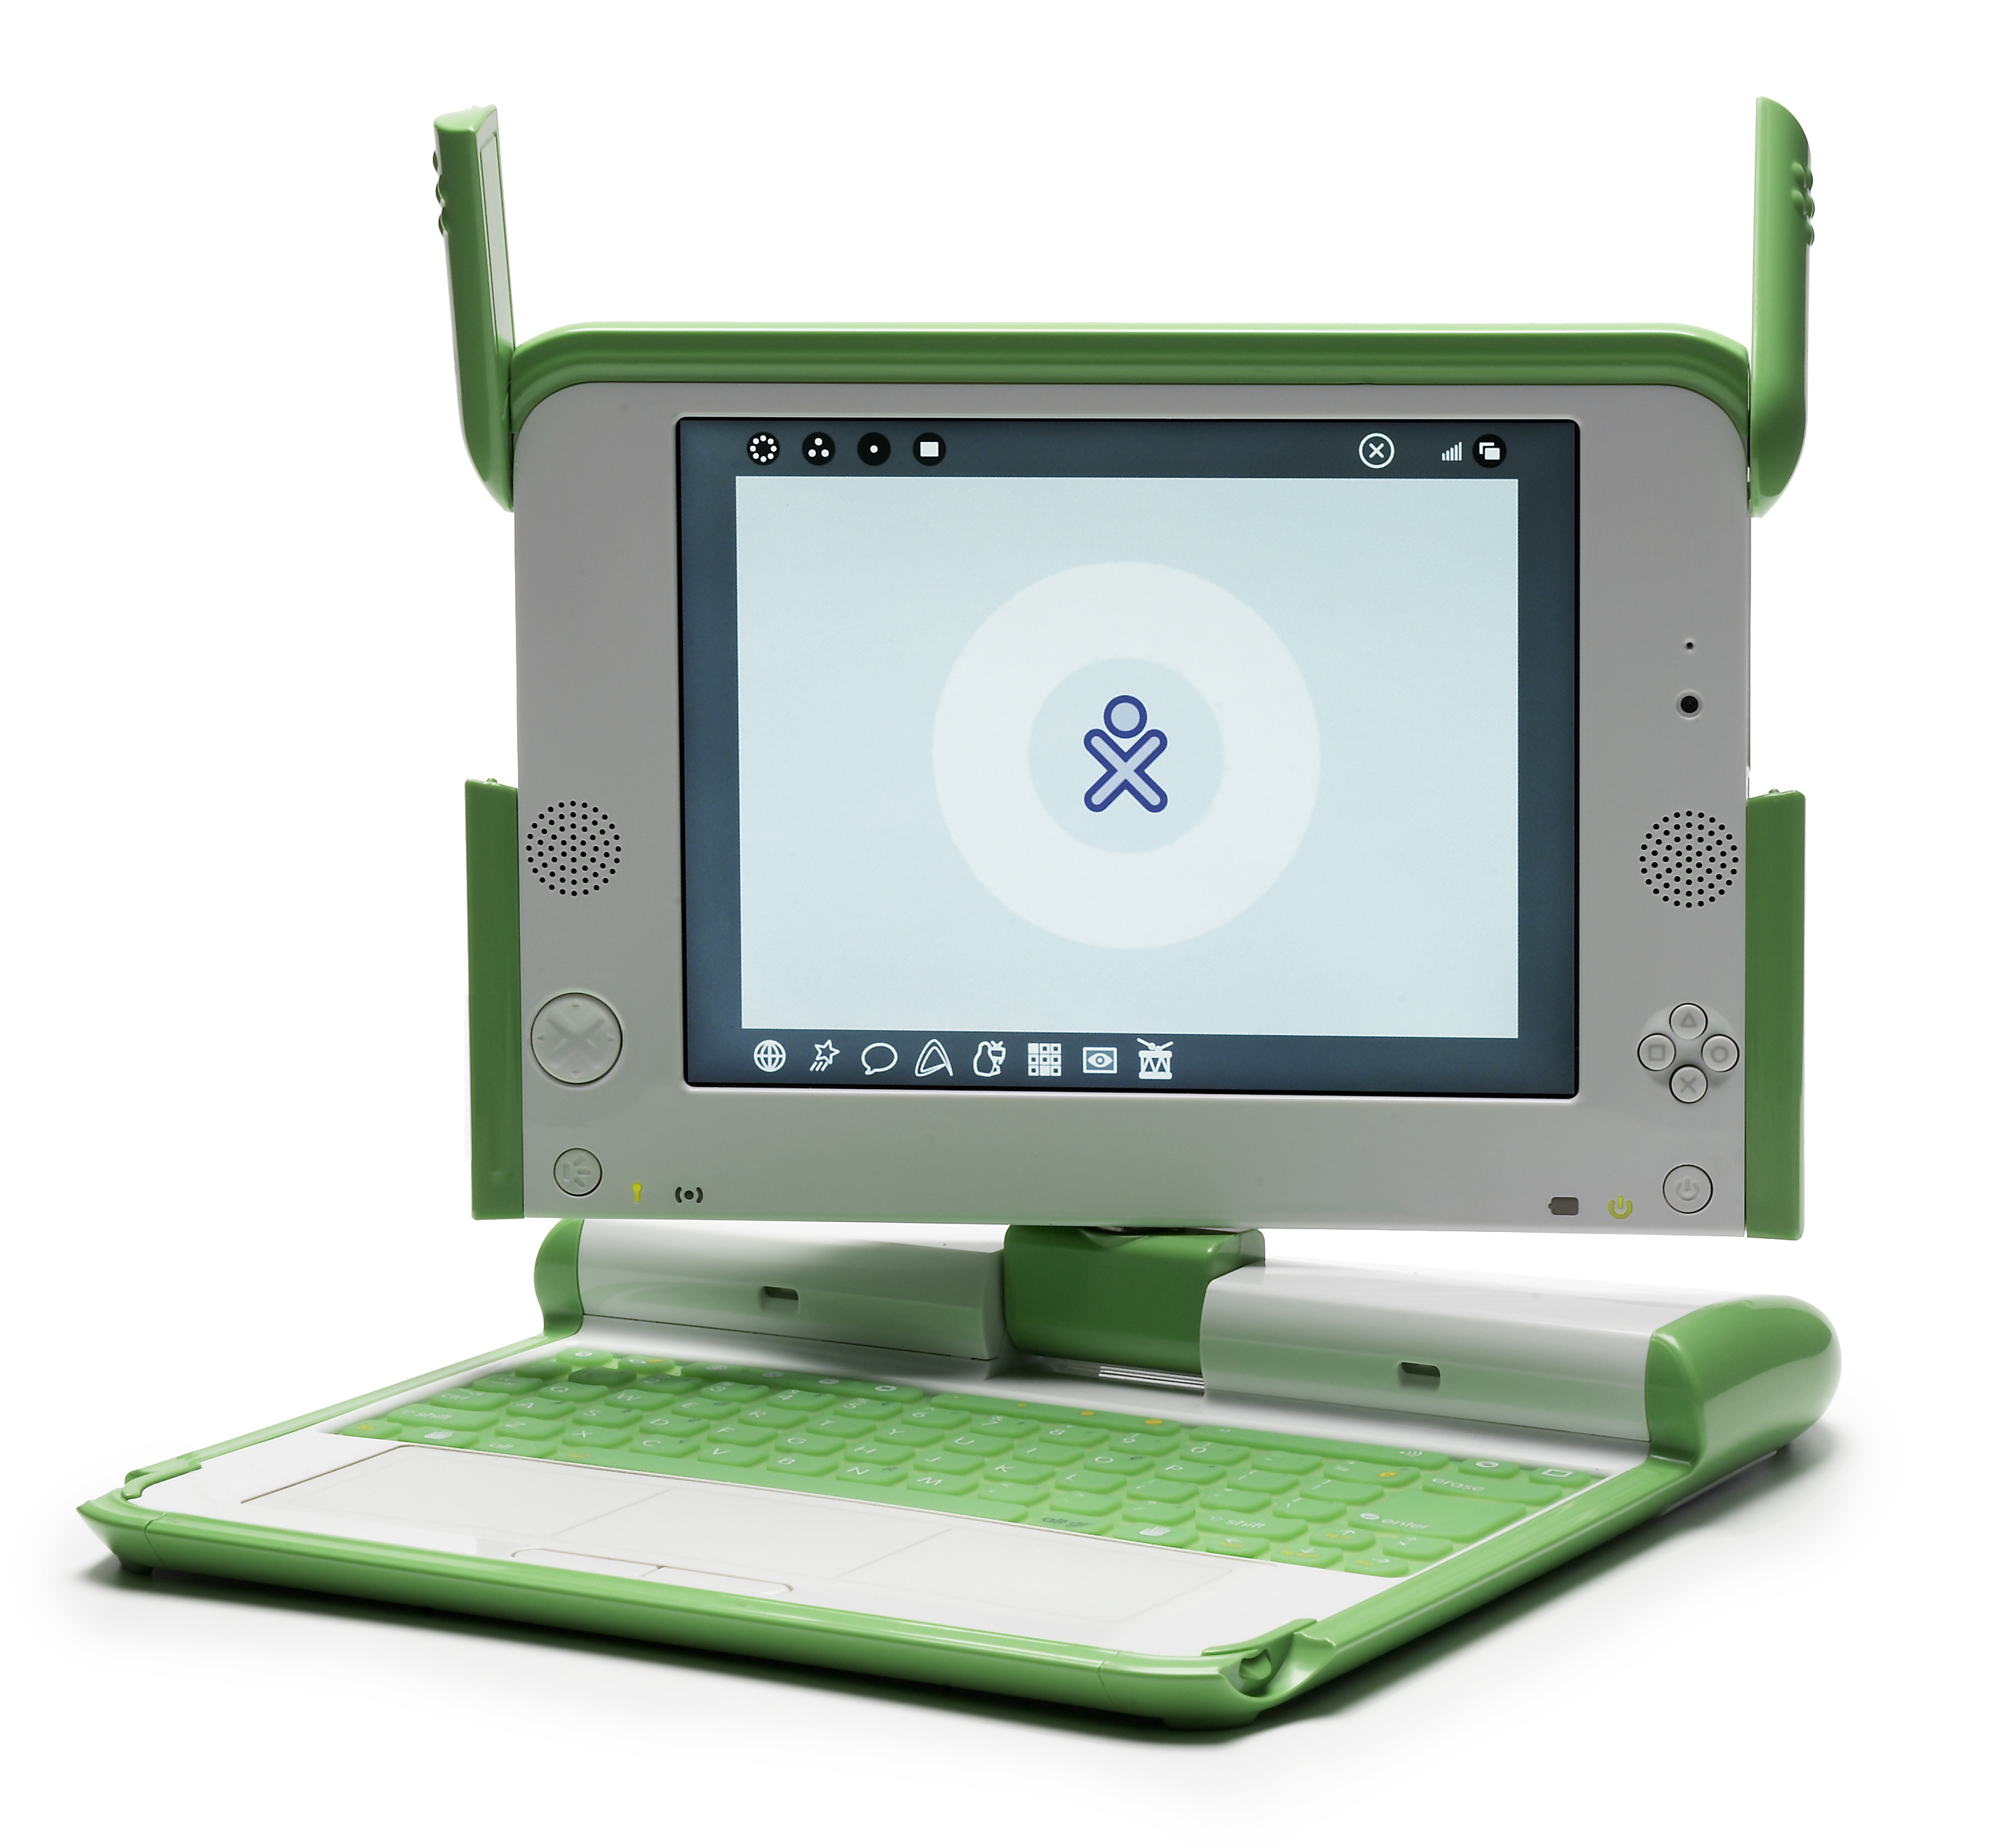
\includegraphics[width=.6\textwidth]{../resources/illustrations/olpc2}
  \caption{XO : ordinateur OLPC}
\end{figure}
\begin{minipage}{.5\linewidth}
  \begin{figure}[H]
    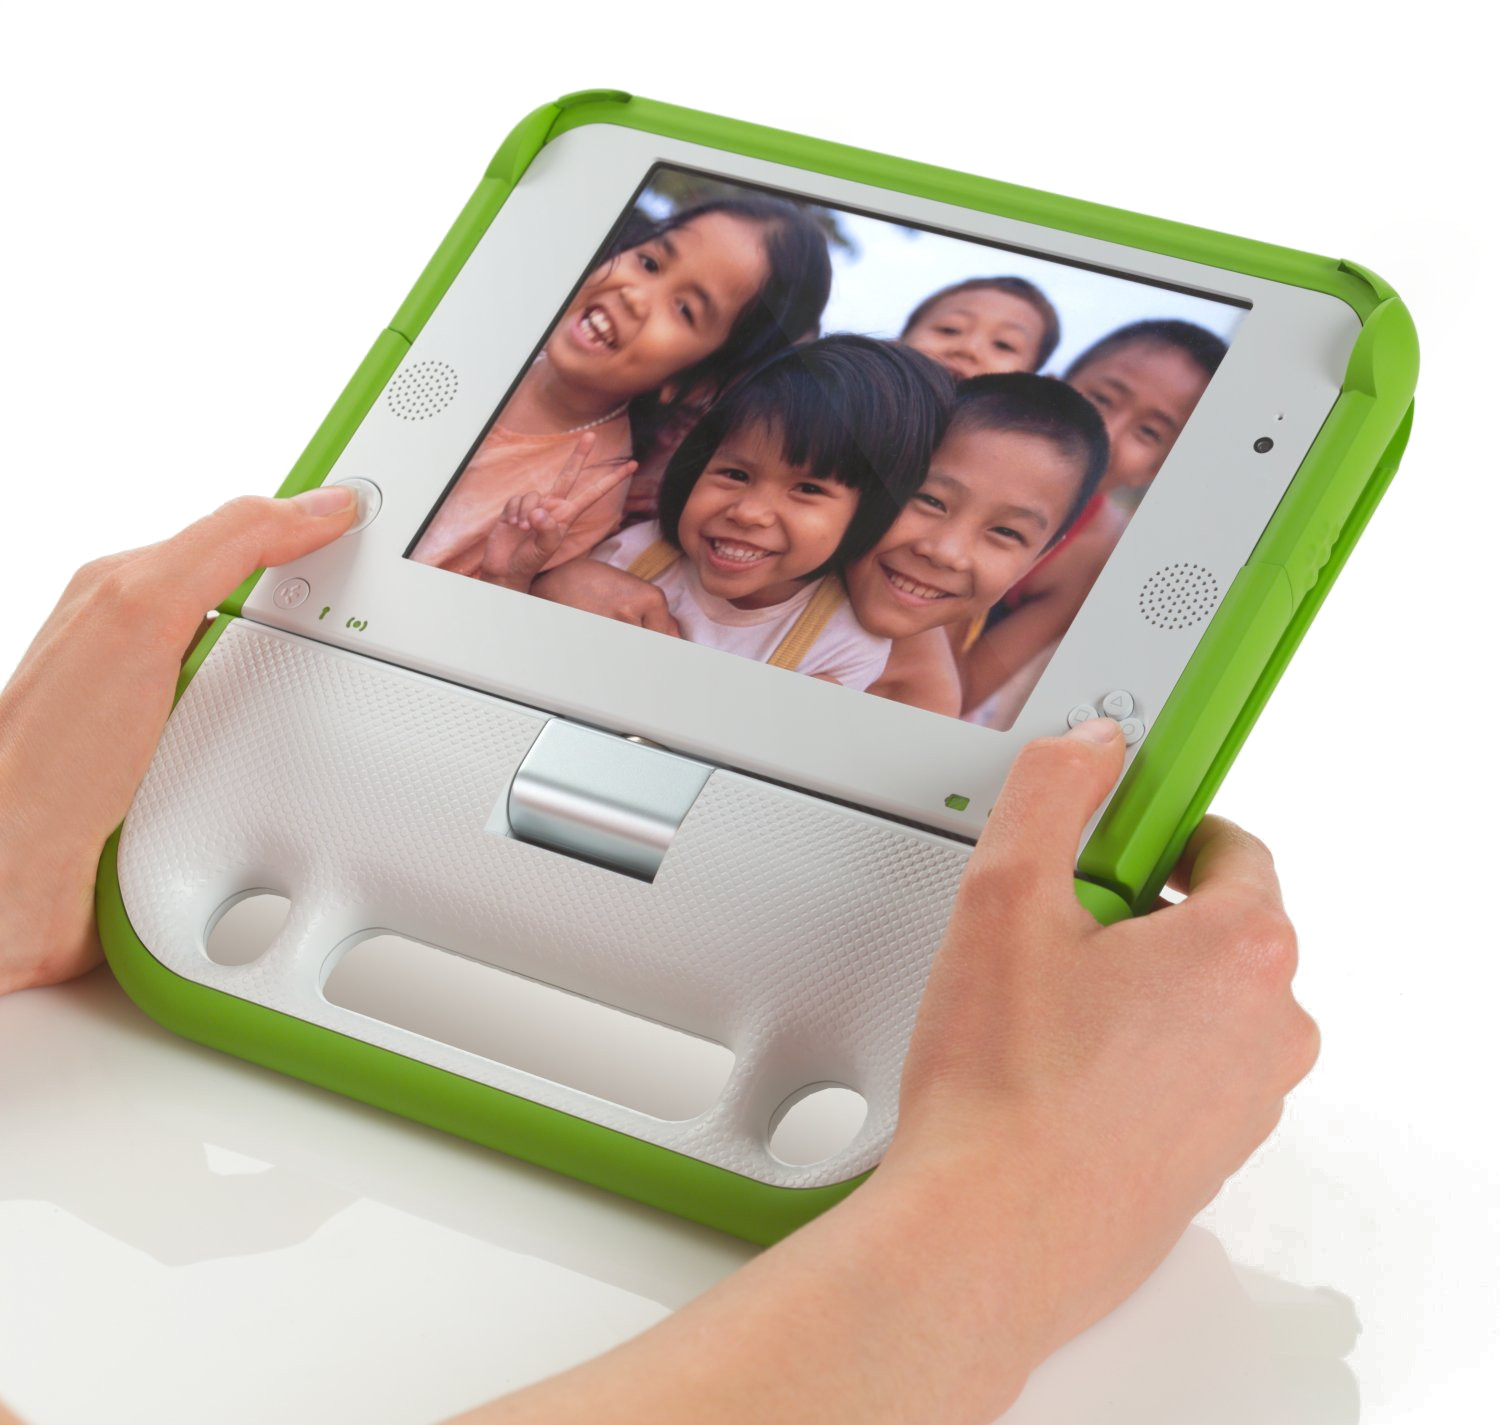
\includegraphics[width=\textwidth]{../resources/illustrations/olpc1}
    \caption{XO : mode Tablet}
  \end{figure}
\end{minipage}
\begin{minipage}{.5\linewidth}
  \begin{figure}[H]
    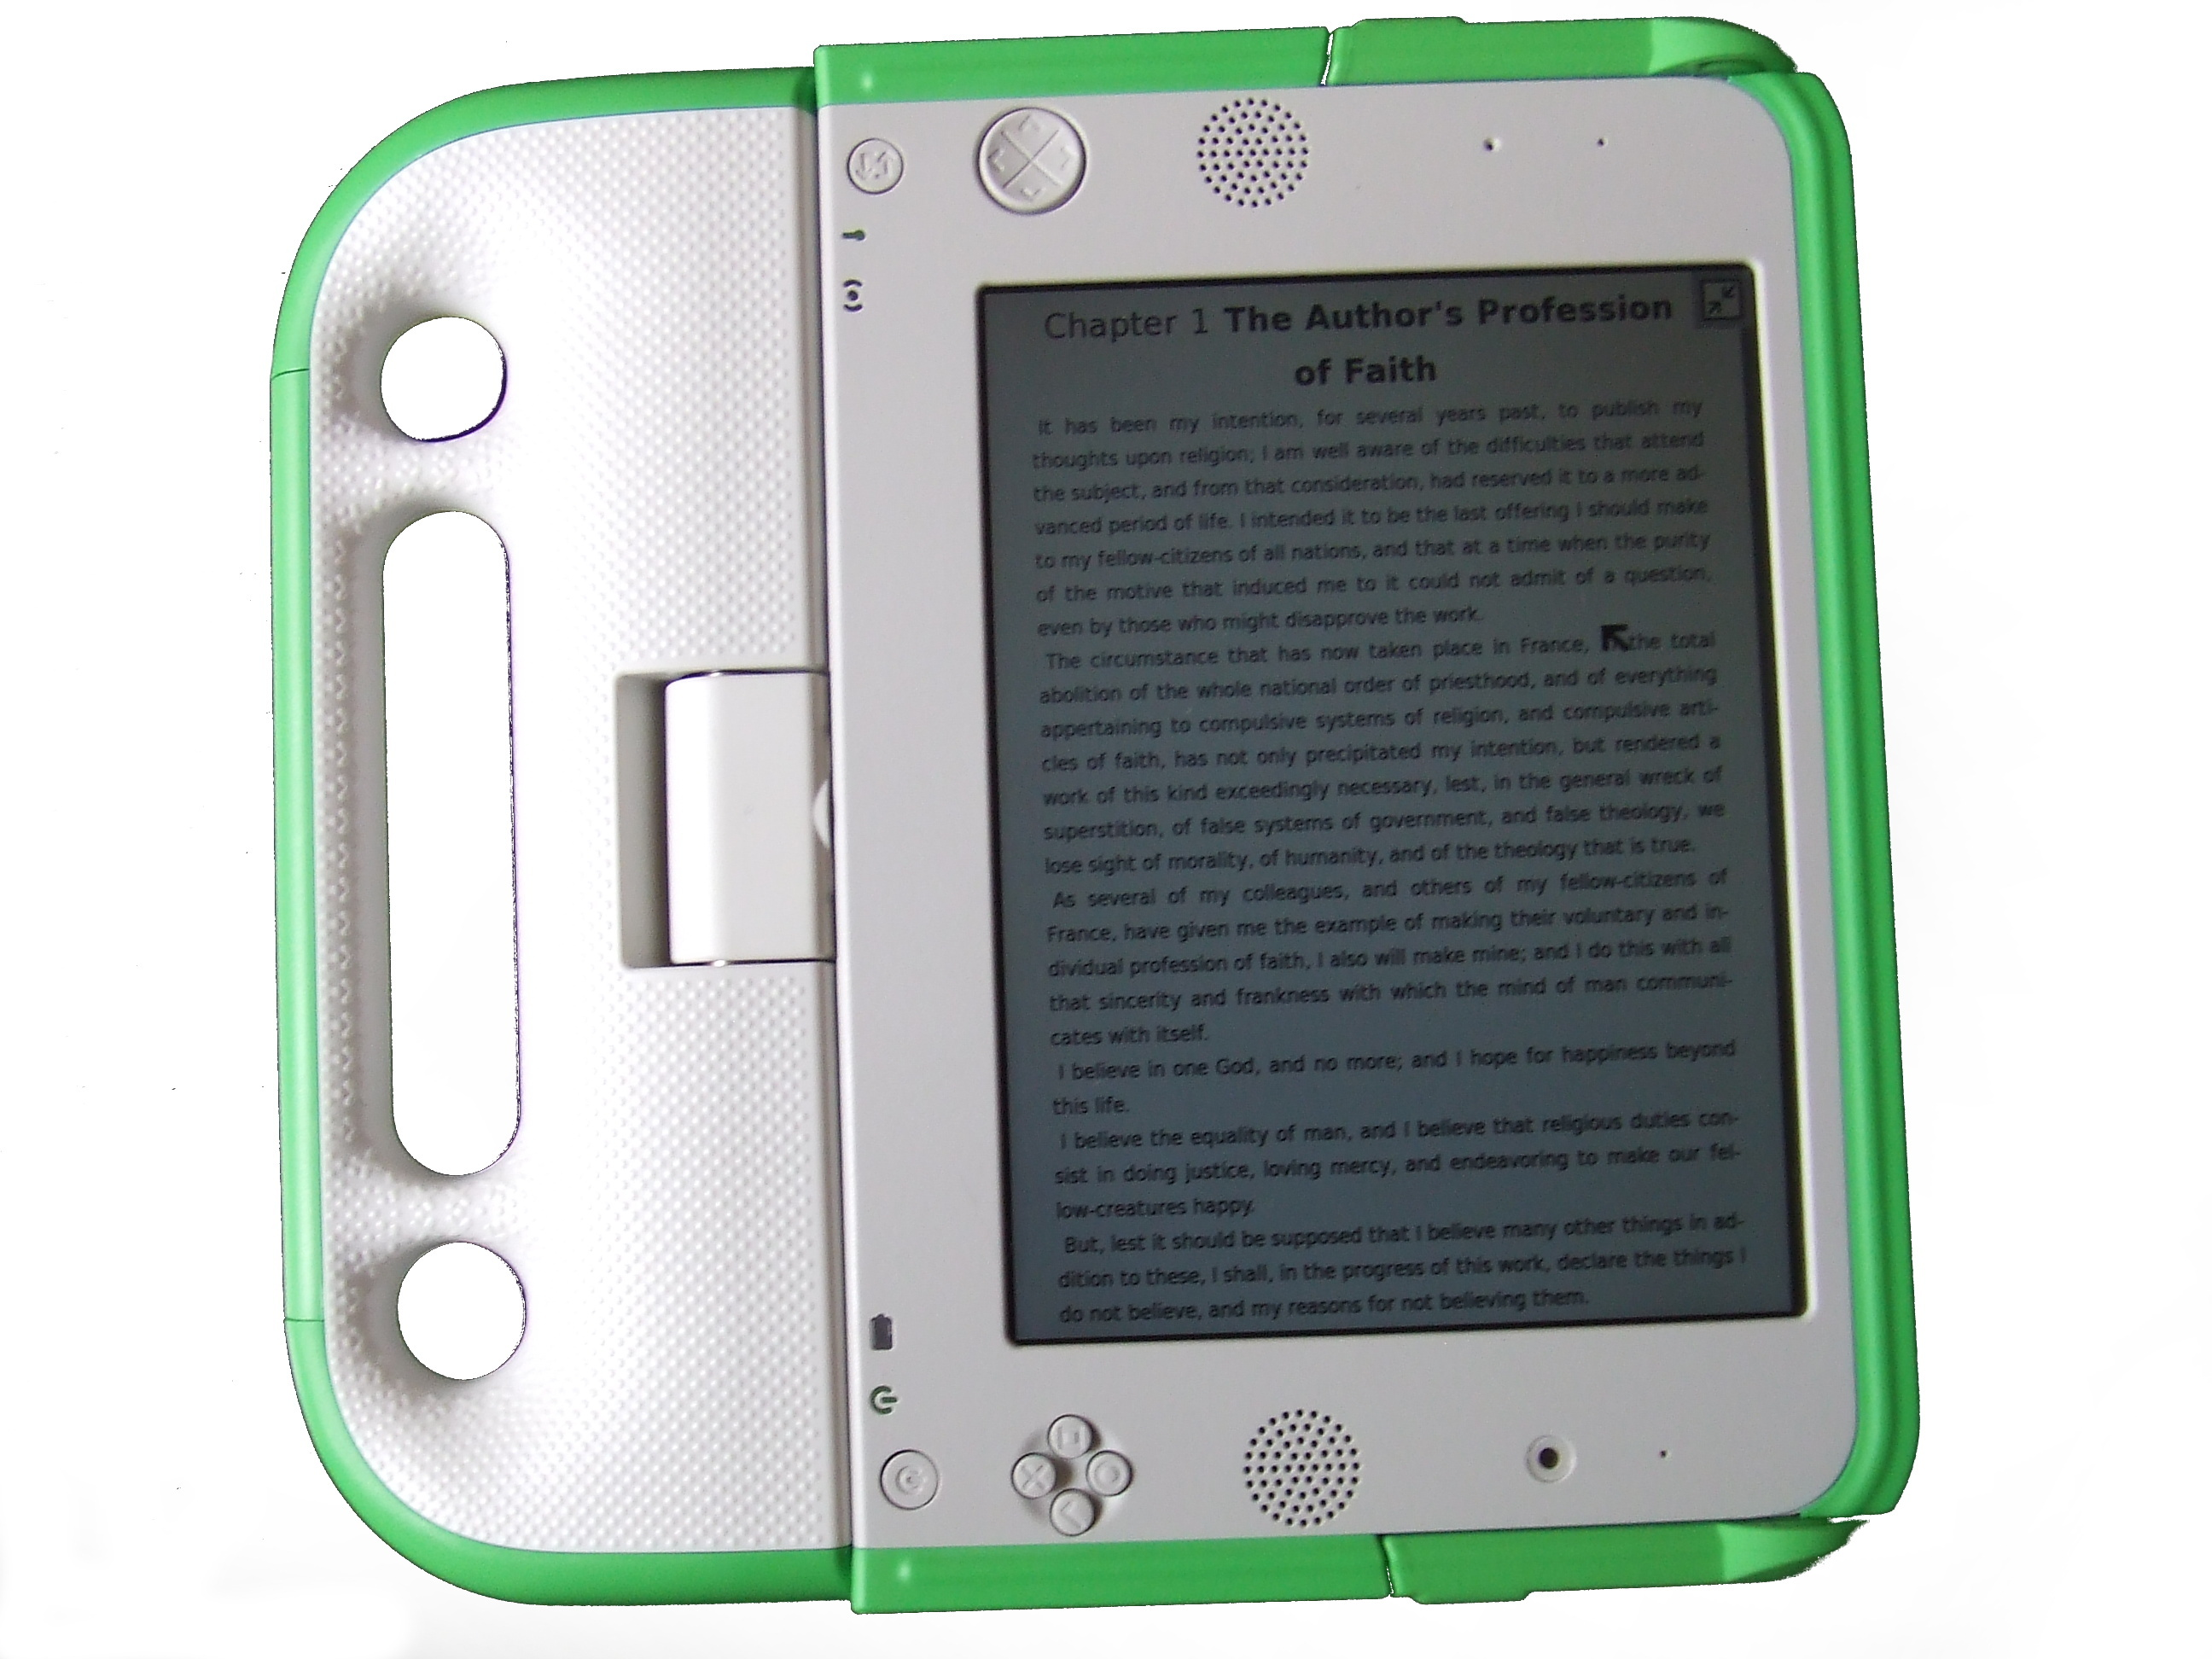
\includegraphics[width=\linewidth]{../resources/illustrations/olpc_display}
    \caption{XO : écran e-paper}
  \end{figure}
\end{minipage}

\section{Hole in the wall}
\textit{Hole in the wall}

\chapter{Solutions}
\label{chap:solutions}

Les initiatives prises exposées dans les chapitres~\ref{chap:initialivespublic} et~\ref{chap:initialisations} pages~\pageref{chap:initialivespublic} et~\pageref{chap:initialivespublic} mettent en évidence des solutions concrètes applicables au modèle éducatif. Celles-ci s'appliquent à deux niveaux : le contenu des enseignements, et la méthode d'enseignement.

\section{Contenu de l'enseignement}
\subsection{Utilisation des NTIC}
Le premier point résident dans la formation aux NTIC\footnote{NTIC : Nouvelles Technologies de l'Information et de la Communication.}. Cet enseignement est en partie déjà dispensé par par le B2I et C2I (voir chapitre~\ref{chap:initialivespublic} page~\pageref{chap:initialivespublic}). Vivant dans une société où l'intégration sociale et professionnelle passe par ces nouvelles formes de communications, il est essentiel d'apprendre aux élèves l'utilisation de ces technologies. L'enseignement se décompose en plusieurs points :

\begin{description}
  \item[Environnement de travail] : manipulation d'un environnement de travail informatisé, gestion et organisation des fichiers, sécuriser ses fichiers.
  \item[Production et exploitation de documents] : formation à l'utilisation d'une suite bureautique et production HTML.
  \item[Recherche d'information] : utilisation des moteurs de recherches, apprendre à mesurer la qualité et la fiabilité d'un document en ligne.
  \item[Collaboration] : envoi / réception d'emails, utilisation d'outils collaboratifs.
\end{description}

Soulignons tout de même l'aspect très technique de cette formation.

\subsection{Manipulation d'images}
Le sujet de cet enseignement peut paraître moins évident. Cependant, il part du fait que nous vivons dans une société où l'image est ultra présente : télévision, internet, magazines, et même dans la rue. L'image est présente dans tous les médias, et particulièrement dans le marketing et la publicité. La nécessité d'une formation en deux point s'impose donc :

\begin{description}
  \item[Lecture d'images] : former à l'analyse d'images, comprendre ce qu'elle signifie où ce que le concepteur à voulu qu'elle exprime, comprendre les principaux mécanismes de trucages et manipulation d'images. Coté prévention face aux images.
  \item[Manipulation d'images] : créer / éditer des images afin de permettre aux élèves de se rendre compte par eux même de la puissance du traitement de l'image.
\end{description}

\subsection{Prévention aux risques}
Actuellement très peu de prévention face au risques que représentent les nouveaux moyens de communication sont données aux élèves. À l'heure où les plus jeunes possèdent déjà de nombreux profils en lignes (réseaux sociaux, blogs, etc.) il semble nécessaire d'informer des dangers liés à l'image qui nous représente au travers de ces plateformes d'échange, et cela dès les premières années de scolarisation.

Des mises en garde pourraient êtres données sur plusieurs plans :

\begin{description}
  \item[Image] : préservation de son image sur Internet, savoir les limites de ce qu'on peut mettre en ligne et partager.
  \item[Vie privée] : garantir la notion de vie privée sur Internet rejoint le point précédent. Apprendre à analyser comment les données personnelles des plateformes en ligne sont partagées, avec qui, et comment limiter ces accès.
  \item[Ventes de données personnelles] : sensibilisation au marketing lié à la vente de données personnelles, à la lecture des condition générales d'utilisation, etc.
\end{description}

\section{Méthode d'enseignement}

Les initiatives présentées dans le chapitre~\ref{chap:initialivesautres} page~\pageref{chap:initialivesautres} sont plus ou moins fortement basées sur une méthode d'apprentissage : le \og constructionnisme \fg{}, qui est lui même fondé sur les principes du constructivisme de Piaget.

\subsection{Le constructivisme}
\begin{minipage}[H]{0.3\linewidth}
  \begin{figure}[H]
  \centering
  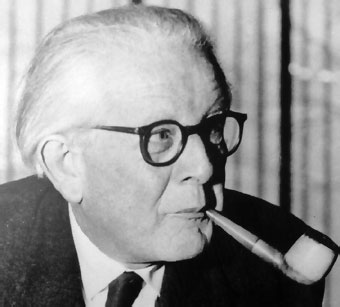
\includegraphics[width=0.8\textwidth]{../resources/illustrations/piaget}
  \caption{Jean Piaget}
  \end{figure}
\end{minipage}
\begin{minipage}[H]{0.7\linewidth}
Jean Piaget, né en 1886 à Neuchâtel et décédé en 1980 à Genève, est connu pour ses travaux en psychologie du comportement. Il est à l'origine du constructivisme et des stades de l'évolution individuelle, qu'il a développé dès 1923 en réaction au Béhaviorisme.
\end{minipage}

\subsubsection{Béhaviorisme}
Le béhaviorisme est un terme inventé par John Broadus Watson. Ce mouvement étudie la psychologie en se limitant qu'aux comportements observables. Il arrive ainsi à un schéma de Stimulus~$\Rightarrow$~Réponse.

Burrhus Frederic Skinner a également travaillé sur le béhaviorisme dans les années 1950. Il y introduit de nouvelles notions comme le conditionnement opérant, révisant ainsi le schéma de Watson en prenant en compte l'individu comme une \og boite noire \fg{} (Émotions, envies, etc.). On obtient donc le schéma suivant : Stimulus~$\Rightarrow$~Individu~$\Rightarrow$~Réponse.

Selon un tel schéma, l'éducation pourra se produire en procédant par instructions répétées (stimuli) et restitution lors de contrôles écrits (réponses).

\subsubsection{Constructivisme}
Le constructivisme affirme que nous ne percevons pas de copies exactes de ce que l'on perçoit. Chacun construit ses propres concepts en fonction de ce qu'il perçoit. En accord avec cette vision, l'éducation se fera en confrontant l'apprenant à des problème difficiles mais réalisables, en le guidant mais sans lui fournir de méthode précise (voir figures~\ref{fig:behaviorisme_vs_constructivisme_illu} et~\ref{fig:behaviorisme_vs_constructivisme_dessin}).

\begin{figure}[H]
  \centering
  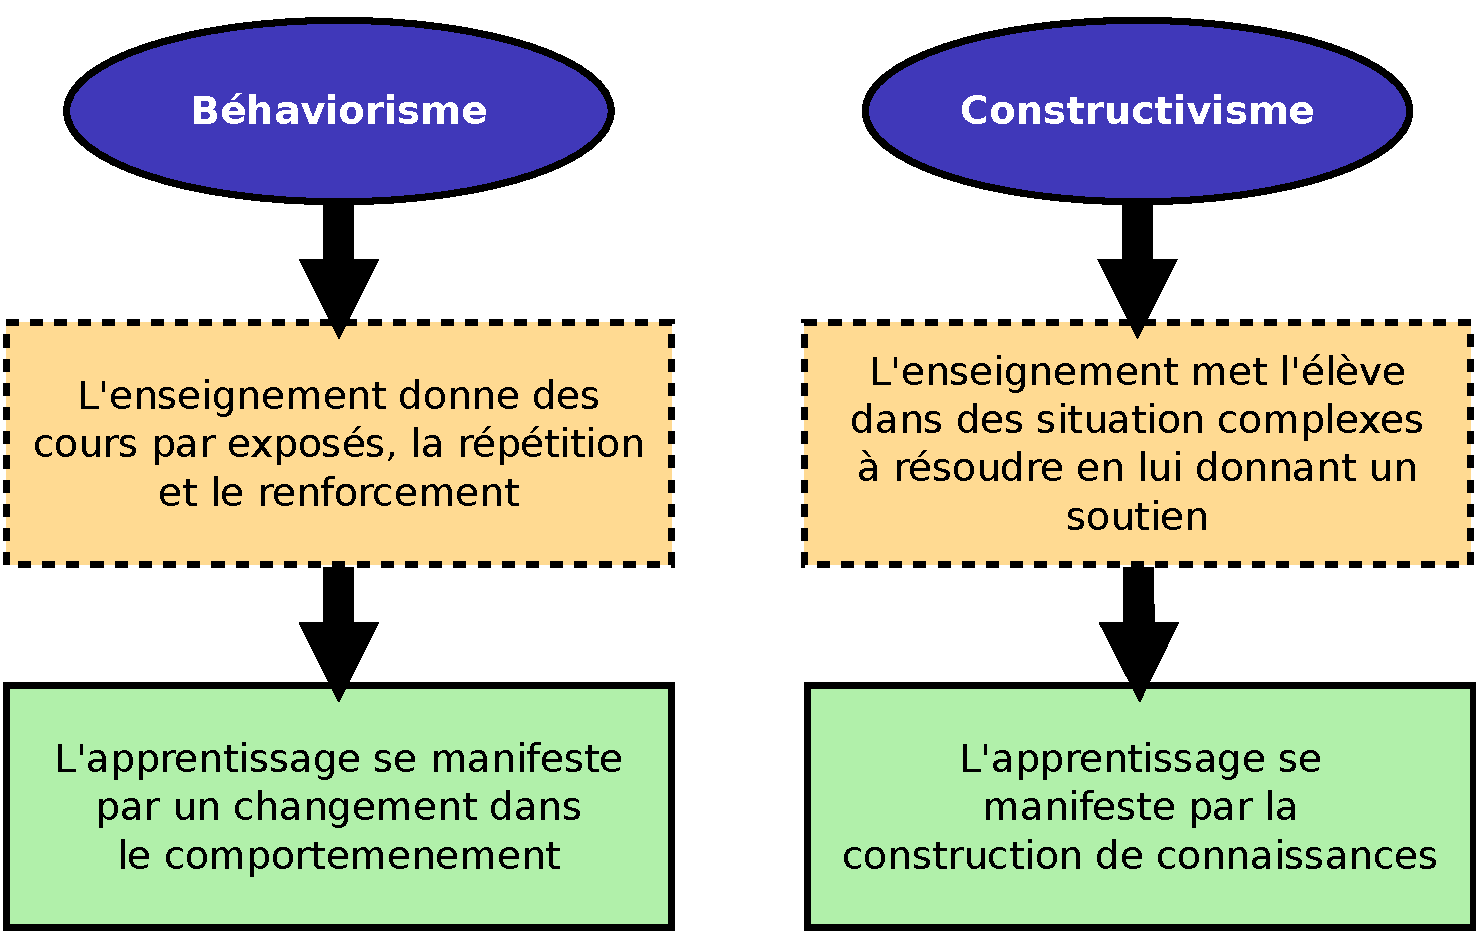
\includegraphics[width=\textwidth]{../resources/illustrations/behaviorisme_constructivisme}
  \caption{Méthode d'apprentissage, béhaviorisme vs. constructivisme}
  \label{fig:behaviorisme_vs_constructivisme_illu}
\end{figure}
\begin{figure}[H]
  \centering
  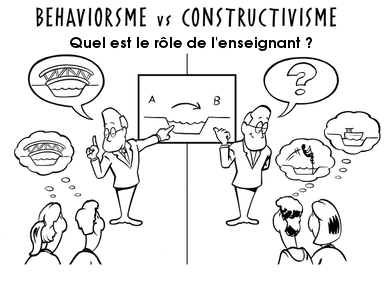
\includegraphics[width=\textwidth]{../resources/illustrations/behaviorisme_vs_constructivisme}
  \caption{Dessin humoristique, béhaviorisme vs. constructivisme}
  \label{fig:behaviorisme_vs_constructivisme_dessin}
\end{figure}